\section{Processing Pipeline}
\label{sec:processing_pipeline}

Having defined the system hardware and sensor configurations, the next step is to establish the processing methodology that transforms raw sensor outputs into reliable odometry estimates.  
The proposed pipeline follows a modular structure, where each stage addresses a specific task: aligning radar frames through rigid-body transformations, merging dual-sensor data, filtering unreliable detections, clustering meaningful structures, and finally estimating ego-motion using Iterative Closest Point (ICP).  

The overall data flow is illustrated in Fig.~\ref{fig:dual_radar_pipeline}, which summarizes how radar and IMU measurements are progressively refined before contributing to odometry estimation.  
This organization enables stepwise validation, as each module can be evaluated independently before integration into the complete system.  

The following subsections present the mathematical formulations and algorithmic logic of each module in detail, supported by block diagrams to illustrate the transformations applied at each stage.  
By combining radar Doppler measurements with orientation inputs from the IMU, the pipeline is designed to deliver robust odometry even in environments where conventional vision- or LiDAR-based methods fail.

\vspace{0.5em}
\subsection{Rigid-Body Transformation}  

Each radar sensor in the dual-radar configuration is physically mounted with a specific orientation and tilt relative to the vehicle's forward direction.
To ensure a common frame of reference for all points, it is necessary to compensate for:

\begin{itemize}
    \item \textbf{Yaw rotation}: due to angled placement ($\pm30^\circ$) of the radar modules.
    \item \textbf{Pitch tilt}: due to upward mounting tilt ($15^\circ$), which must be compensated to recover horizontal geometry.
    \item \textbf{Sensor offset}: due to the physical separation of the radar sensors in the horizontal axis (X-axis).
\end{itemize}

The transformation from radar to vehicle coordinates is expressed as:
\begin{equation}
    \vec{p}_{\text{veh}} = R_{\text{yaw}} \cdot R_{\text{pitch}} \cdot \vec{p}_{\text{radar}} + \vec{T}
    \label{eq:radar_to_vehicle_transform_short}
\end{equation}

These corrections ensured that detections from both radars overlapped coherently, avoiding duplicated or misaligned clusters.  
Without them, raw dual-sensor data appeared inconsistent, particularly when fusing Doppler-based velocity estimates.  
After applying yaw, pitch, and translation adjustments, the fused point cloud served as a stable input for clustering, odometry, and tracking.

\vspace{0.5em}
\subsubsection{Yaw Correction (Z-axis Rotation)}
The radar sensors are rotated relative to the vehicle frame:

\begin{itemize}
    \item Radar A (Left): Mounted at $+30^\circ$ yaw $\Rightarrow$ compensated with $-30^\circ$ rotation.
    \item Radar B (Right): Mounted at $-30^\circ$ yaw $\Rightarrow$ compensated with $+30^\circ$ rotation.
\end{itemize}

The 2D rotation in the XY-plane is defined as:
\[
\begin{bmatrix}
x' \\
y' \\
z'
\end{bmatrix}
=
\begin{bmatrix}
\cos(\theta) & -\sin(\theta) & 0 \\
\sin(\theta) & \cos(\theta) & 0 \\
0 & 0 & 1
\end{bmatrix}
\begin{bmatrix}
x \\
y \\
z
\end{bmatrix}
\]

where $\theta = \pm30^\circ$ depending on the sensor.

\begin{figure}[!htbp]
    \centering
    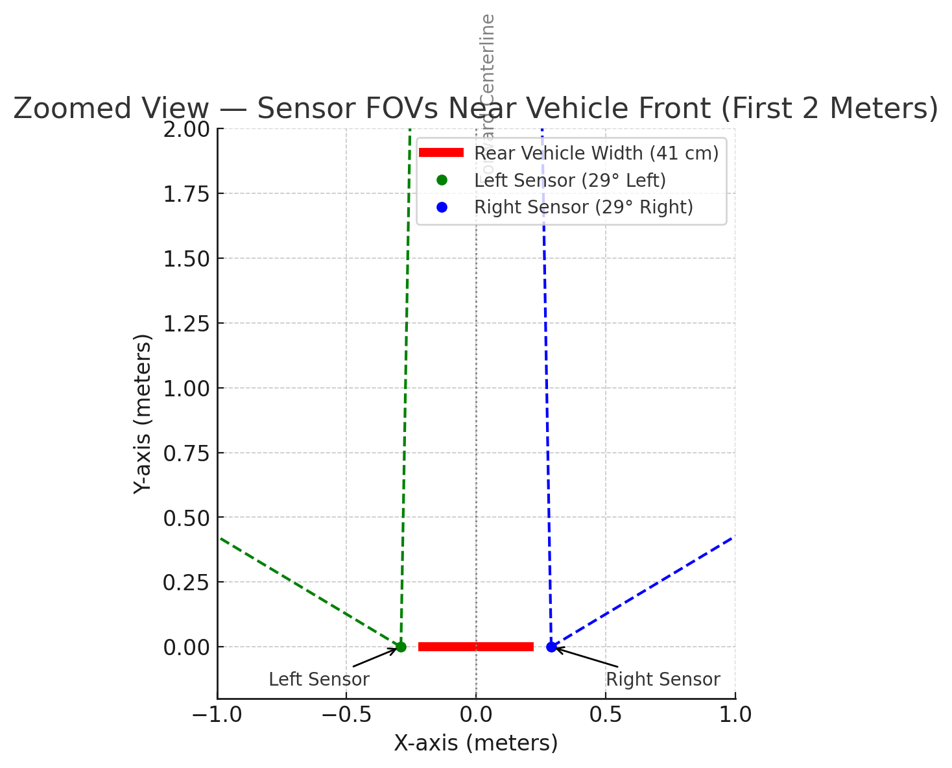
\includegraphics[width=0.8\linewidth]{images/SensorsRotation.png}
    \caption{Simulation of yaw rotation of sensors around the Z-axis ($\pm30^\circ$).}
    \label{fig:z_axis_rotation}
\end{figure}

\begin{figure}[!htbp]
    \centering
    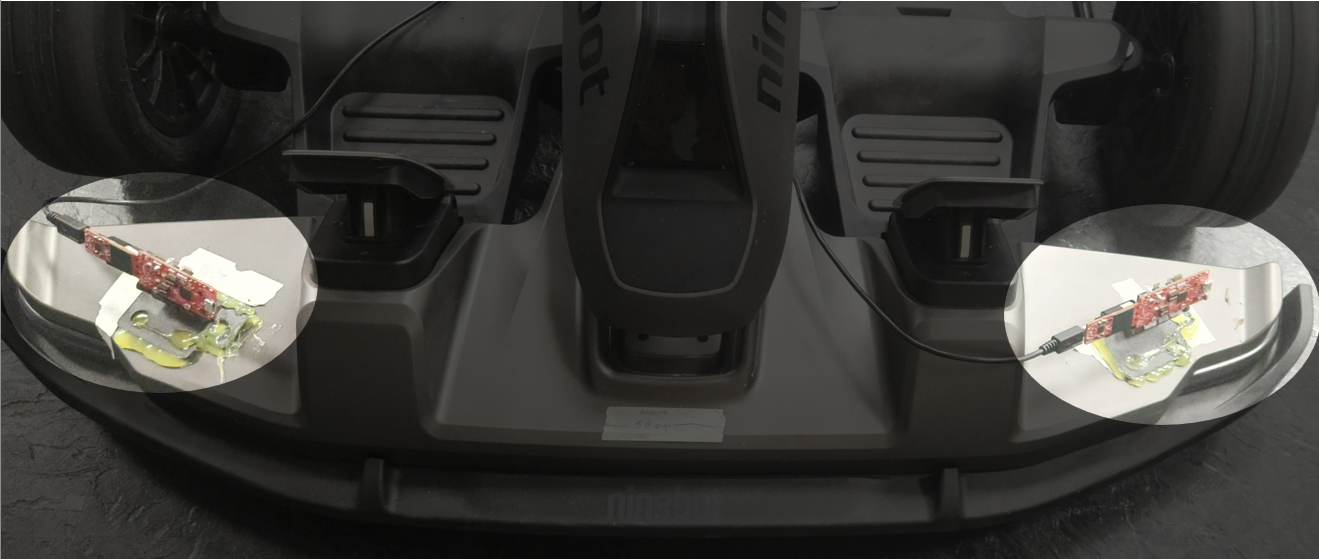
\includegraphics[width=0.8\linewidth]{images/vehicleRadarYawRotationHighlited.png}
    \caption{Real-world implementation of yaw rotation in the vehicle.}
    \label{fig:vehicleRadarYawRotation}
\end{figure}

\newpage
The yaw angles of $\pm30^\circ$ were selected through a combination of physical measurement and simulation of the sensor field of view (FOV).  
Using the vehicle chassis centerline as a reference, the mounted sensors were visually measured to exhibit a yaw of approximately $28$--$32^\circ$ outward (see Fig.~\ref{fig:vehicleRadarYawRotation}), which confirmed the intended target of $30^\circ$ opening from the vehicle center.  
This estimate was further cross-checked in simulation by plotting the radar FOV using the TI Demo Visualizer, which allows configuration of the theoretical horizontal FOV from its default $90^\circ$ down to $60^\circ$ or $30^\circ$ respectfully.  
\begin{comment}
    Add picture of this validation
\end{comment}
The $60^\circ$ configuration was adopted as it provides improved angular resolution while discarding irrelevant detections outside the useful sector.  
Within this setting, the $\pm30^\circ$ mounting maximizes the combined coverage of the dual-radar system, while creating a small blind zone of approximately $4$~m directly in front of the vehicle.  
This trade-off was deliberately accepted to ensure the widest effective overlap of both radars for odometry tasks.

\vspace{0.5em}
\subsubsection{Pitch Compensation (X-axis Rotation)}
Since the radar sensors are tilted upward by $15^\circ$, a corrective rotation around the X-axis is applied to bring the points back to a horizontal perspective: 

\[
\begin{bmatrix}
x' \\ y' \\ z'
\end{bmatrix}
=
\begin{bmatrix}
1 & 0 & 0 \\
0 & \cos(\phi) & -\sin(\phi) \\
0 & \sin(\phi) & \cos(\phi)
\end{bmatrix}
\begin{bmatrix}
x \\ y \\ z
\end{bmatrix}
\]

where $\phi = -15^\circ$ (negative to reverse the upward tilt).

\begin{figure}[!htbp]
    \centering
    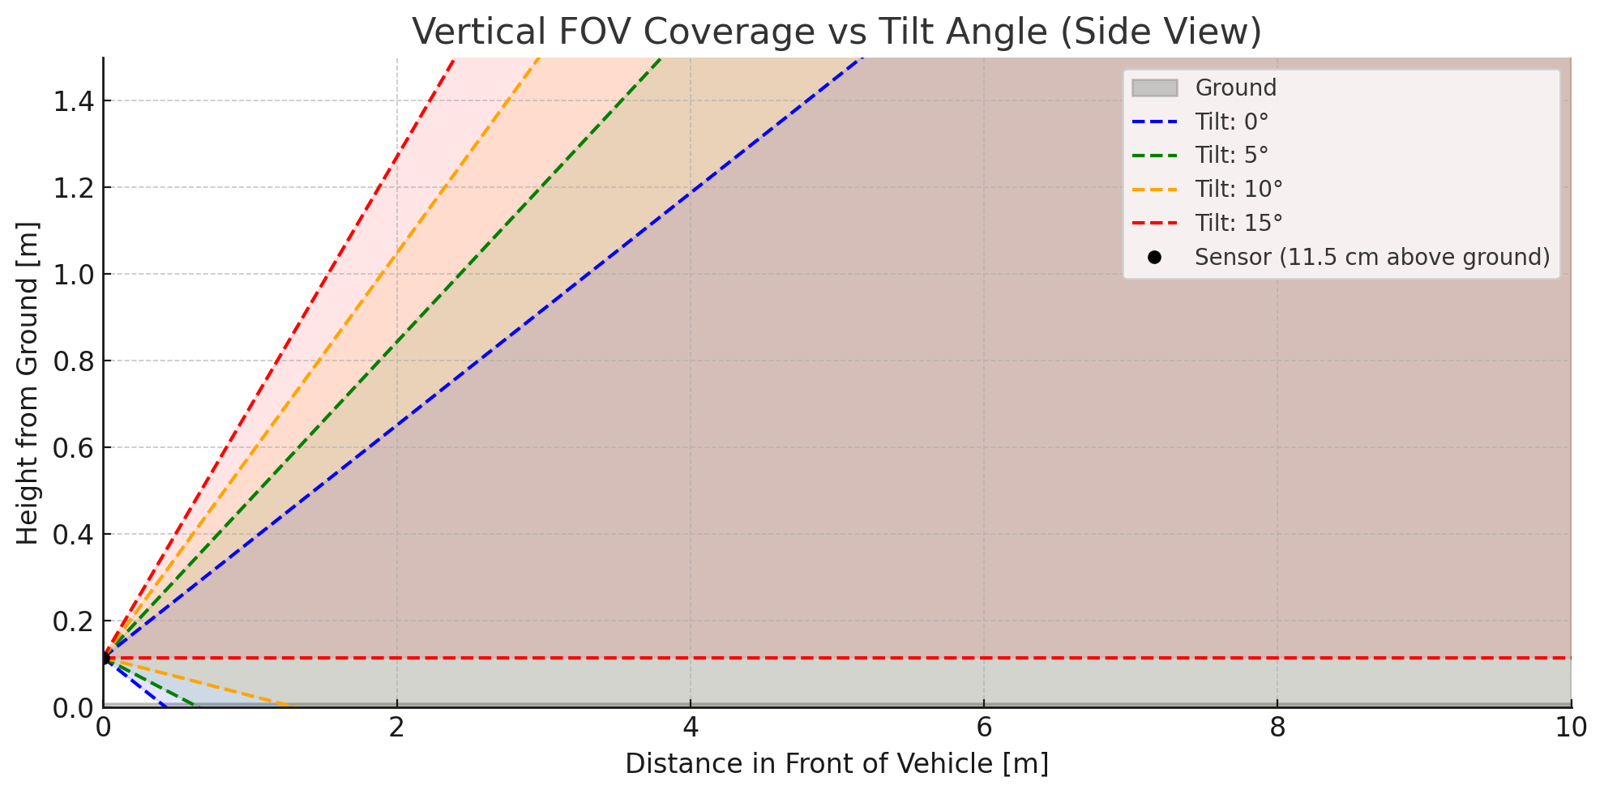
\includegraphics[width=0.8\linewidth]{images/TiltSensor.png}
    \caption{Pitch compensation for $15^\circ$ upward tilt.}
    \label{fig:x_axis_rotation}
\end{figure}

The upward tilt of $15^\circ$ was introduced to minimize clutter from the ground plane.  
With the sensor's vertical FOV of approximately $30^\circ$, this configuration reduced spurious reflections while maintaining sufficient detection of obstacles at the intended height range.  
Both the yaw and pitch choices were tested through simulation and validated in real-world mounting experiments (Figures~\ref{fig:z_axis_rotation}, \ref{fig:vehicleRadarYawRotation}, \ref{fig:x_axis_rotation}, \ref{fig:vehicleYawTilt}).

\begin{figure}[!htbp]
    \centering
    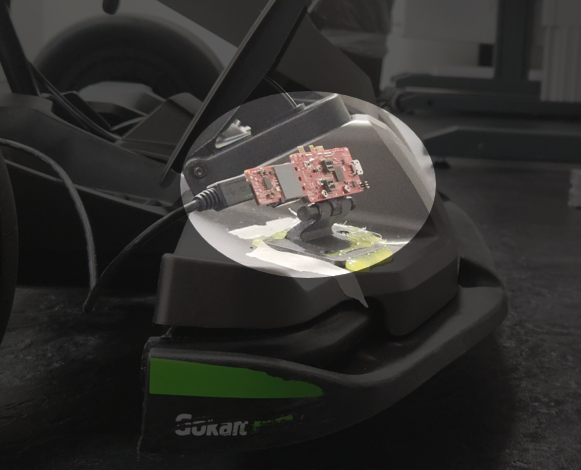
\includegraphics[width=0.8\linewidth]{images/vehicleRadarTiltRotation.png}
    \caption{Real-world implementation of radar tilt ($15^\circ$ upward).}
    \label{fig:vehicleYawTilt}
\end{figure}

\subsubsection{X-Axis Offset Compensation}
After rotation, each sensor's point cloud was translated along the X-axis to align with the vehicle's center:
\begin{itemize}
    \item Radar A: $x \leftarrow x - 0.32$ meters
    \item Radar B: $x \leftarrow x - 0.28$ meters
\end{itemize}

This translation ensured both sensors were aligned in a common vehicle-centric frame.

\begin{figure}[!htbp]
    \centering
    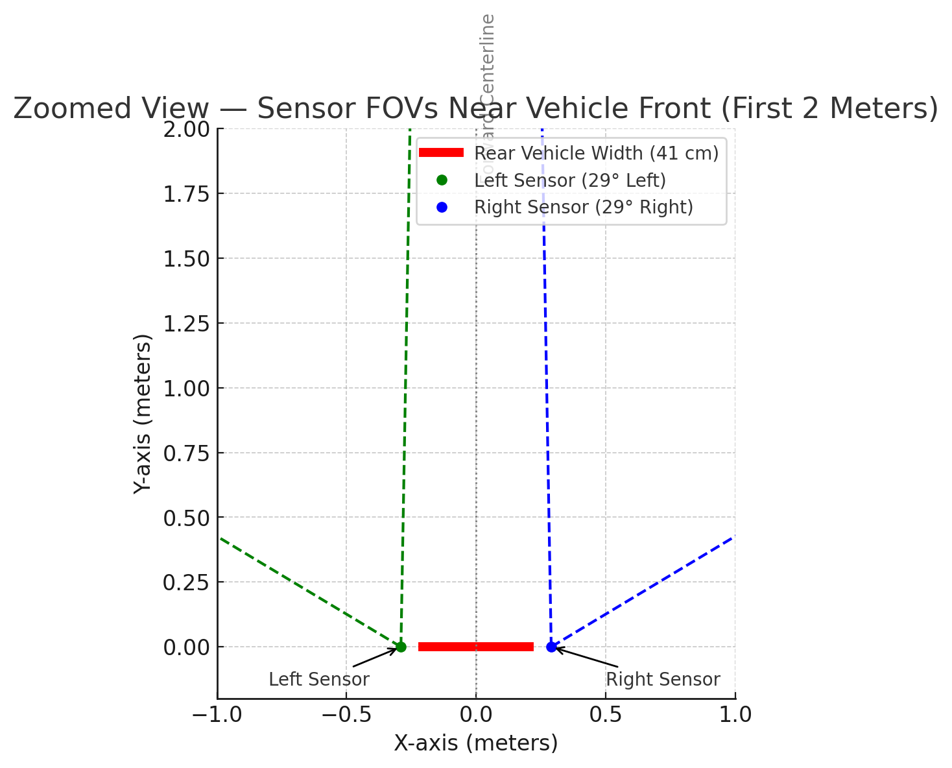
\includegraphics[width=0.8\linewidth]{images/RotationSensor.png}
    \caption{Final extrinsic configuration combining yaw, pitch, and translation.}
    \label{fig:extrinsics}
\end{figure}

A yaw rotation \( R_{\text{yaw}} \) was first implemented, followed by a pitch correction \( R_{\text{pitch}} \), and finally a translation vector \( \vec{t} \) was applied to account for the physical position of the sensors with respect to the vehicle's coordinate origin.

The full transformation can be expressed as:

\begin{equation}
T_{\text{veh}} = R_{\text{yaw}} \cdot R_{\text{pitch}} \cdot \vec{p}_{\text{radar}} + \vec{T}
\label{eq:radar_to_vehicle_transform}
\end{equation}

Where:
\begin{itemize}
    \item \( \vec{p}_{\text{radar}} \) is a radar point in sensor coordinates.
    \item \( R_{\text{yaw}} \) is a 2D rotation around the vertical axis ($\pm30^\circ$).
    \item \( R_{\text{pitch}} \) corrects for the upward sensor tilt ($-15^\circ$).
    \item \( \vec{T} \) is the translation vector.
\end{itemize}

\subsubsection{Summary of Extrinsics}
\begin{itemize}
    \item \textbf{Left radar:} yaw $+30^\circ$, pitch $-15^\circ$, translation $(-0.32, 0, 0)$.
    \item \textbf{Right radar:} yaw $-30^\circ$, pitch $-15^\circ$, translation $(-0.28, 0, 0)$.
\end{itemize}

This extrinsic calibration ensures that dual-radar data is expressed in a coherent vehicle-centric frame, which is critical for downstream modules such as clustering, odometry, and obstacle tracking.

\vspace{0.5em}
\subsection{Radar Merge}  
\indent Once each radar's detections were transformed into the common vehicle frame, the two datasets were merged into a single unified point cloud per frame.  
This step ensured that detections from both radars contributed consistently to the pipeline.  

This fusion improves both density and coverage, particularly in regions where the individual radar fields of view overlap.  
It also reduces ambiguity during clustering, since targets detected by both sensors reinforce one another once aligned.  

The effect of merging is visualized in Fig.~\ref{fig:radar_merge}, where the independent point clouds (top) are combined into a single dataset (bottom).  

\begin{figure}[!htbp]
    \centering
    \begin{subfigure}[t]{0.8\linewidth}
        \centering
        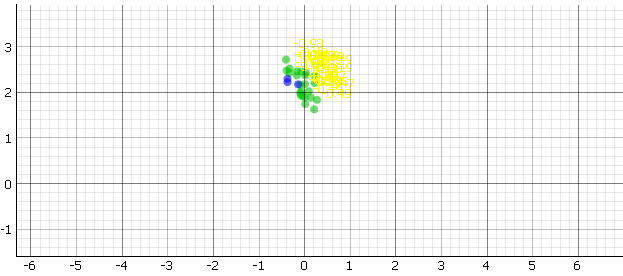
\includegraphics[width=\linewidth]{images/AFTERdualSensorCalib_2mts.png}
        \caption{Independent point clouds before merging.}
    \end{subfigure}
    \vfill
    \begin{subfigure}[t]{0.8\linewidth}
        \centering
        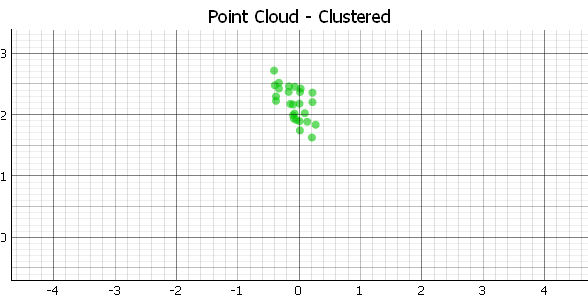
\includegraphics[width=\linewidth]{images/AFTERdualSensorCalibCluster_2mts.png}
        \caption{Unified point cloud after merging.}
    \end{subfigure}
    \caption{Radar merge process: alignment of calibrated detections into a single dataset. (a) Radar A = blue, Radar B = green. (b) Merged point cloud.}
    \label{fig:radar_merge}
\end{figure}
